\documentclass[a0,landscape]{a0poster}
\usepackage{hyperref}
\usepackage{multicol} % This is so we can have multiple columns of text side-by-side
\columnsep=80pt % This is the amount of white space between the columns in the poster
%\columnseprule=2pt % This is the thickness of the black line between the columns in the poster

\usepackage[svgnames]{xcolor} % Specify colors by their 'svgnames', for a full list of all colors available see here: http://www.latextemplates.com/svgnames-colors

\usepackage{times} % Use the times font
%\usepackage{palatino} % Uncomment to use the Palatino font

\usepackage{graphicx} % Required for including images
%\graphicspath{{C:/Users/huawei/Desktop/images/}} % Location of the graphics files
\usepackage{booktabs} % Top and bottom rules for table
\usepackage[font=small,labelfont=bf]{caption} % Required for specifying captions to tables and figures
\usepackage{amsfonts, amsmath, amsthm, amssymb} % For math fonts, symbols and environments
\usepackage{wrapfig} % Allows wrapping text around tables and figures
\usepackage[english]{babel}
\usepackage[scale=2]{ccicons}
\usepackage{picture}
\usepackage{tikz}
\usepackage[absolute,overlay]{textpos}
\usepackage{spot}
\usepackage{tabularx}
\usepackage{multirow}
\usepackage{caption}
\usepackage{subcaption}
\usepackage{spot}
\usepackage{floatrow}
\usepackage{setspace}
\usepackage{listings}
\usepackage[english]{babel}


\usetikzlibrary{calc, positioning, shapes.arrows}
\definecolor{title}{RGB}{20,68,199}
\definecolor{comp}{RGB}{35, 99, 70}
\definecolor{inc}{RGB}{191, 13, 43}
\definecolor{oldlavender}{rgb}{0.47, 0.41, 0.47}
\definecolor{command}{rgb}{153,112,171}
\definecolor{comment}{rgb}{90,174,97}


\lstset{language=R,
	basicstyle=\small\ttfamily,
	stringstyle=\color{blue},
	%otherkeywords={0,1,2,3,4,5,6,7,8,9},
	morekeywords={TRUE,FALSE, clean\_iat, d\_plot, d\_distr},	
	deletekeywords={<, -, data, \_, order, plot, col},
	keywordstyle=\color{purple}\bfseries,
	commentstyle=\color{green!40!blue},
}

\begin{document}

%----------------------------------------------------------------------------------------
%	POSTER HEADER 
%----------------------------------------------------------------------------------------

% The header is divided into two boxes:
% The first is 75% wide and houses the title, subtitle, names, university/organization and contact information
% The second is 25% wide and houses a logo for your university/organization or a photo of you
% The widths of these boxes can be easily edited to accommodate your content as you see fit

\begin{minipage}[b]{\linewidth}
	\begin{textblock*}{12cm}(10cm,0.5cm)
		
\includegraphics[width=\linewidth]{implicitMeasures.png}\\
	\end{textblock*}
	
	\begin{center}
\veryHuge \textcolor{title}{\textbf{Scoring the implicit:}}
\veryHuge\textcolor{title}{\textbf{The \texttt{implicitMeasures} package}}\\[2cm] % Subtitle	

\LARGE \textbf{Ottavia M. Epifania, Egidio Robusto, \& Pasquale Anselmi}\\[0.5cm] % Author(s)
\Large University of Padova\\[0.4cm] % University/organization
\Large \texttt{marinaottavia.epifania@phd.unipd.it}\\	
	\end{center}

	\begin{textblock*}{12cm}(98cm,0.5cm)
		\begin{tabular}{l}
			\href{https://github.com/OttaviaE/implicitMeasures}{
\includegraphics[width=\linewidth]{github.png}}
		\end{tabular}
	
\end{textblock*}

\end{minipage}
%
%\begin{minipage}[b]{0.25\linewidth}
%\includegraphics[width=3cm]{logo.png}\\
%\end{minipage}

%\vspace{0.5cm} % A bit of extra whitespace between the header and poster content

%----------------------------------------------------------------------------------------
\setlength{\columnseprule}{0.4pt}
 % This is how many columns your poster will be broken into, a portrait poster is generally split into 2 columns

\begin{multicols*}{3}
%----------------------------------------------------------------------------------------
%	ABSTRACT
%----------------------------------------------------------------------------------------

\begin{center}
	\huge \textbf{\textcolor{title}{Introduction}}
\end{center}

\vspace{5mm}
\large
Within the past decades, social sciences have been showing a growing interest for the implicit investigation of attitudes and preference. This was made possible by the advent of what are called implicit measures, among which the Implicit Association Test (IAT) \cite{Greenwald1998} and the Single Category IAT (SC-IAT) \cite{karpinski2006} are the mostly common used ones \cite{review}.
Both tests result in a differential score (the so-called \emph{D-score}) expressing respondents’ bias in performing the categorization task between conditions. While the scoring of the SC-IAT is based on one single algorithm \cite{karpinski2006}, six different algorithms are available for computing the IAT \emph{D-score} \cite{Greenwald2003}.

%Despite that many R packages exist for computing IAT \emph{D-score} algorithms, no packages exist for scoring the SC-IAT. Additionally, majority of existing R packages created for the computation of IAT \emph{D-score} algorithms do not provide all the available algorithms. The packages allowing for the computation of multiple \emph{D-score} algorithms either do not offer the chance to compare their results, or do not disambiguate the specific algorithm they are computing, raising reproducibility issues \cite{ellithorpe2015}. 

\texttt{implicitMeasures} is an \texttt{R} package aimed at providing an easy to use tool to score both the IAT and the SC-IAT, and to easily compare the results obtained with the different \emph{D-score} algorithms. The package basic functioning is illustrated. 


\begin{center}
	\Large \textbf{\textcolor{title}{The Implicit Association Test}}
\end{center}

The IAT is usually composed of seven blocks:

\begin{center}
	\begin{tabular}{llll}
		\multicolumn{4}{c}{IAT structure \label{tab:iat}}\\
		\toprule
		Block & Function & Left response key & Right response key  \\
		\midrule
		\emph{B1} & Practice & Object 1 & Object 2 \\
		\emph{B2} & Practice & \emph{Good} & \emph{Bad} \\
		\textcolor{comp}{\emph{B3}} & \textcolor{comp}{Associative Practice Mapping A} & \textcolor{comp}{Object 1 + \emph{Good}} & \textcolor{comp}{Object 2 + \emph{Bad}} \\
		\textcolor{comp}{\emph{B4} } & \textcolor{comp}{Associative Test Mapping A} & \textcolor{comp}{Object 1 + \emph{Good}} & \textcolor{comp}{Object 2 + \emph{Bad}} \\
		\emph{B5} & Practice & Object 2 & Object 1 \\
		\textcolor{inc}{\emph{B6}} & \textcolor{inc}{Associative Practice Mapping B} & \textcolor{inc}{Object 2 + \emph{Good}} & \textcolor{inc}{Object 1 + \emph{Bad}} \\
		\textcolor{inc}{\emph{B7}} & \textcolor{inc}{Associative Test Mapping B} & \textcolor{inc}{Object 2 + \emph{Good}} & \textcolor{inc}{Object 1 + \emph{Bad} }\\
		\bottomrule
	\end{tabular}
\end{center}

\vspace{3mm}

The computation of the IAT \emph{D-score} is rather easy but 6 different algorithms are available:

\begin{tabular}{lll}
	\large	
	$\text{\emph{D-score}} = \frac{M_{\text{MappingA}} - M_{\text{MappingB}}}{sd_{\text{pooled}}}$
	    & &	\begin{tabular}{lll}
		\multicolumn{3}{c}{IAT \emph{D-score} algorithms}\\
		\toprule
		\emph{D-score} & Error Replacement & Lower tail treatment \\
		\midrule
		\emph{D1} & Built-in & No \\ 
		\emph{D2} & Built-in & $<$ 400 ms \\ 
		\emph{D3} & Mean + 2 \emph{sd} & No \\ 
		\emph{D4} & Mean + 600 ms & No \\ 
		\emph{D5} & Mean +2 \emph{sd} & $<$ 400 ms \\ 
		\emph{D6} & Mean + 600 ms & $<$ 400 ms \\ 
		\bottomrule
		\multicolumn{3}{l}{\emph{Note:} Trials with rt $>$ 10,000 ms are discarded}\\
	\end{tabular}\\
\end{tabular}

\vspace{3mm}
\begin{center}
	\Large \textbf{\textcolor{title}{The Single Category Implicit Association Test}}
\end{center}

Same assumption, same score computation as the IAT \textbf{BUT} just one target object: 
\begin{center}
	\begin{tabular}{llll}
		\multicolumn{4}{c}{SC-IAT structure \label{tab:sciat}}\\
		\toprule
		Block & Function & Left response key & Right response key  \\
		\midrule
		\emph{B1} & Associative Practice Mapping A & Object 1 + \emph{Good} & \emph{Bad} \\
		\textcolor{comp}{\emph{B2} } & \textcolor{comp}{Associative Test Mapping A} & \textcolor{comp}{Object 1 + \emph{Good}} & \textcolor{comp}{\emph{Bad}} \\
		\emph{B3} & Associative Practice Mapping B & \emph{Good} & Object 1 + \emph{Bad} \\
		\textcolor{inc}{\emph{B4}} & \textcolor{inc}{Associative Test Mapping B} & \textcolor{inc}{ \emph{Good}} & \textcolor{inc}{Object 1 + \emph{Bad} }\\
		\bottomrule
	\end{tabular}
\end{center}

\vspace{3mm}
The SC-IAT \emph{D-score} is computed as the IAT \emph{D-score} by considering just the responses in Blocks \emph{B2} and \emph{B4}. Error responses are replaced by the average response time added with a penalty of 400 ms. Responses faster than 350 ms are discarded. The administration might include a Response Time Window (rtw) at 1,500 ms after which the stimulus disappears and the response is considered a non-response. 



\vfill\null
\columnbreak

\begin{center}
	\huge \textbf{\textcolor{title}{IAT example}}
\end{center}

The examples are based on the toy data set included in \texttt{implicitMeasures} package. 
\begin{lstlisting}
data("raw_data") # load toy data
iat_data <- clean_iat(raw_data, # raw data set 
           sbj_id = "Participant", #Respondents' IDs
           block_id = "blockcode", #Blocks labels
           mapA_practice = "practice.iat.Milkbad", #Label B3
           mapA_test = "test.iat.Milkbad", # Label B4
           mapB_practice = "practice.iat.Milkgood", #Label B6
           mapB_test = "test.iat.Milkgood", #Label B7
           latency_id = "latency", #Response times
           accuracy_id = "correct", #Accuracy responses)
\end{lstlisting}

Function \textbf{\textcolor{purple}{\texttt{clean\_iat()}}} results in a list, in which the first object is a data frame with class \textcolor{purple}{\texttt{iat\_clean}}. This data set can be passed to function \textbf{\textcolor{purple}{\texttt{computeD()}}}: 
\begin{lstlisting}
iat_dscore <- computeD(iat_cleandata[[1]], #iat_clean object
                       Dscore =  "d2") #D-score algorithm
\end{lstlisting}
The object \textbf{\textcolor{purple}{\texttt{iat\_dscore}}} is an object of class \textcolor{purple}{\texttt{dscore}}. This object can be passed to functions \textbf{\textcolor{purple}{\texttt{descript\_d()}}} (i.e., print a table of descirptive statistics of the results, even in \LaTeX), \textbf{\textcolor{purple}{\texttt{IATrel()}}} (i.e., compute teh IAT reliability), and to functions for obtaining graphical representation of the results, either at the individual respondente with function \textbf{\textcolor{purple}{\texttt{d\_plot()}}} or at the sample level with function \textbf{\textcolor{purple}{\texttt{d\_distr()}}}: 
%
\begin{tabular}{c c}
		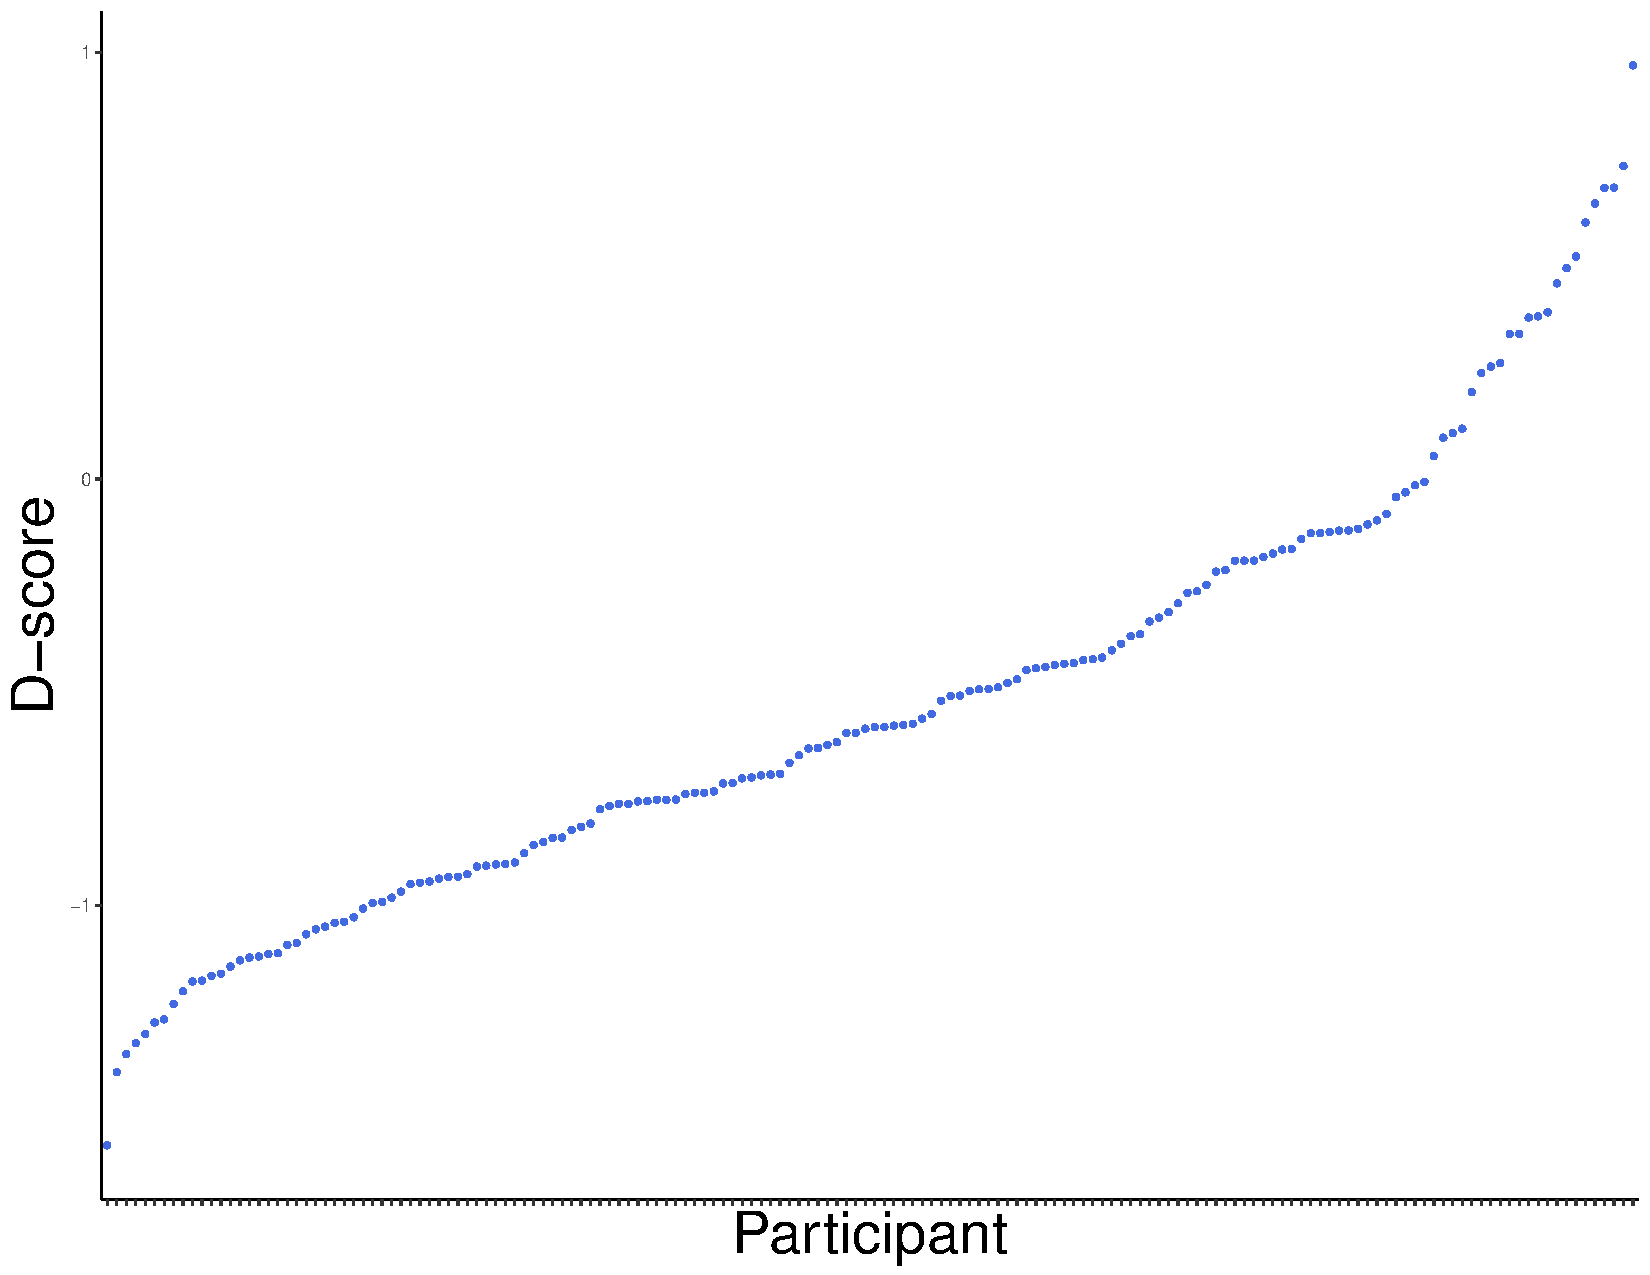
\includegraphics[width=0.5\linewidth]{dplot.pdf}
	&
		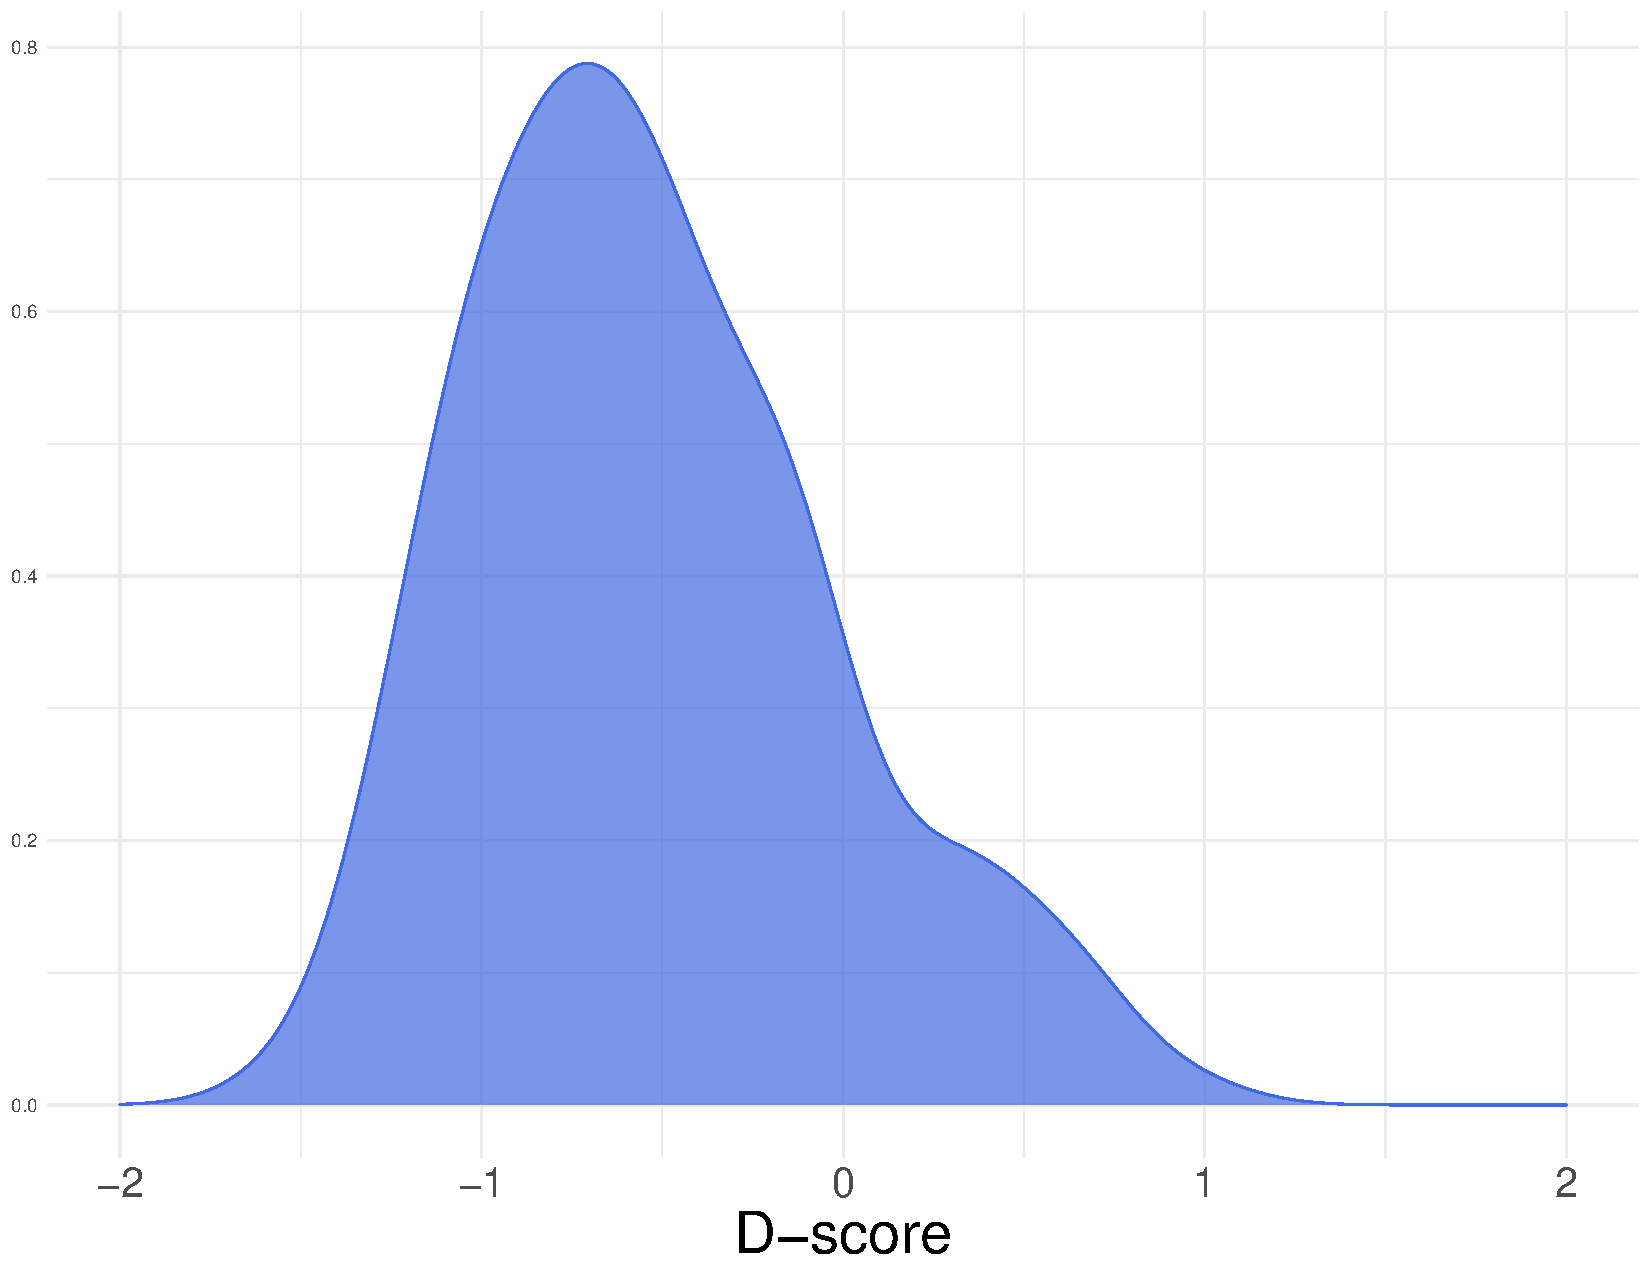
\includegraphics[width=0.5\linewidth]{ddistr.pdf} \\
		\textbf{\textcolor{purple}{\texttt{d\_plot()}}} & \textbf{\textcolor{purple}{\texttt{d\_distr()}}}\\
\end{tabular}

\vspace{3mm}

The object with class \textcolor{purple}{\texttt{iat\_clean}} can also be passed to function \textcolor{purple}{\texttt{multi\_dscore()}}, which simultaneously compute multiple \emph{D-score} algorithms: 
\begin{lstlisting}
multiple_scores <- multi_dscore(iat_cleandata[[1]], 
	            ds = `error-inflation`) #Which algorithm?
\end{lstlisting}

Function \textbf{\textcolor{purple}{\texttt{multiple\_scores()}}} results in a list containing a data set with a number of columns equal to the number of computed alrgorithms plus a column for respondnents' IDs and a graph with the distribution resulting from the different algorithms: 


	\begin{tabular}{l}
		\begin{lstlisting}
		multiple_scores$graph # Only select the graphical output
		\end{lstlisting}\\
		
		\multicolumn{1}{c}{ 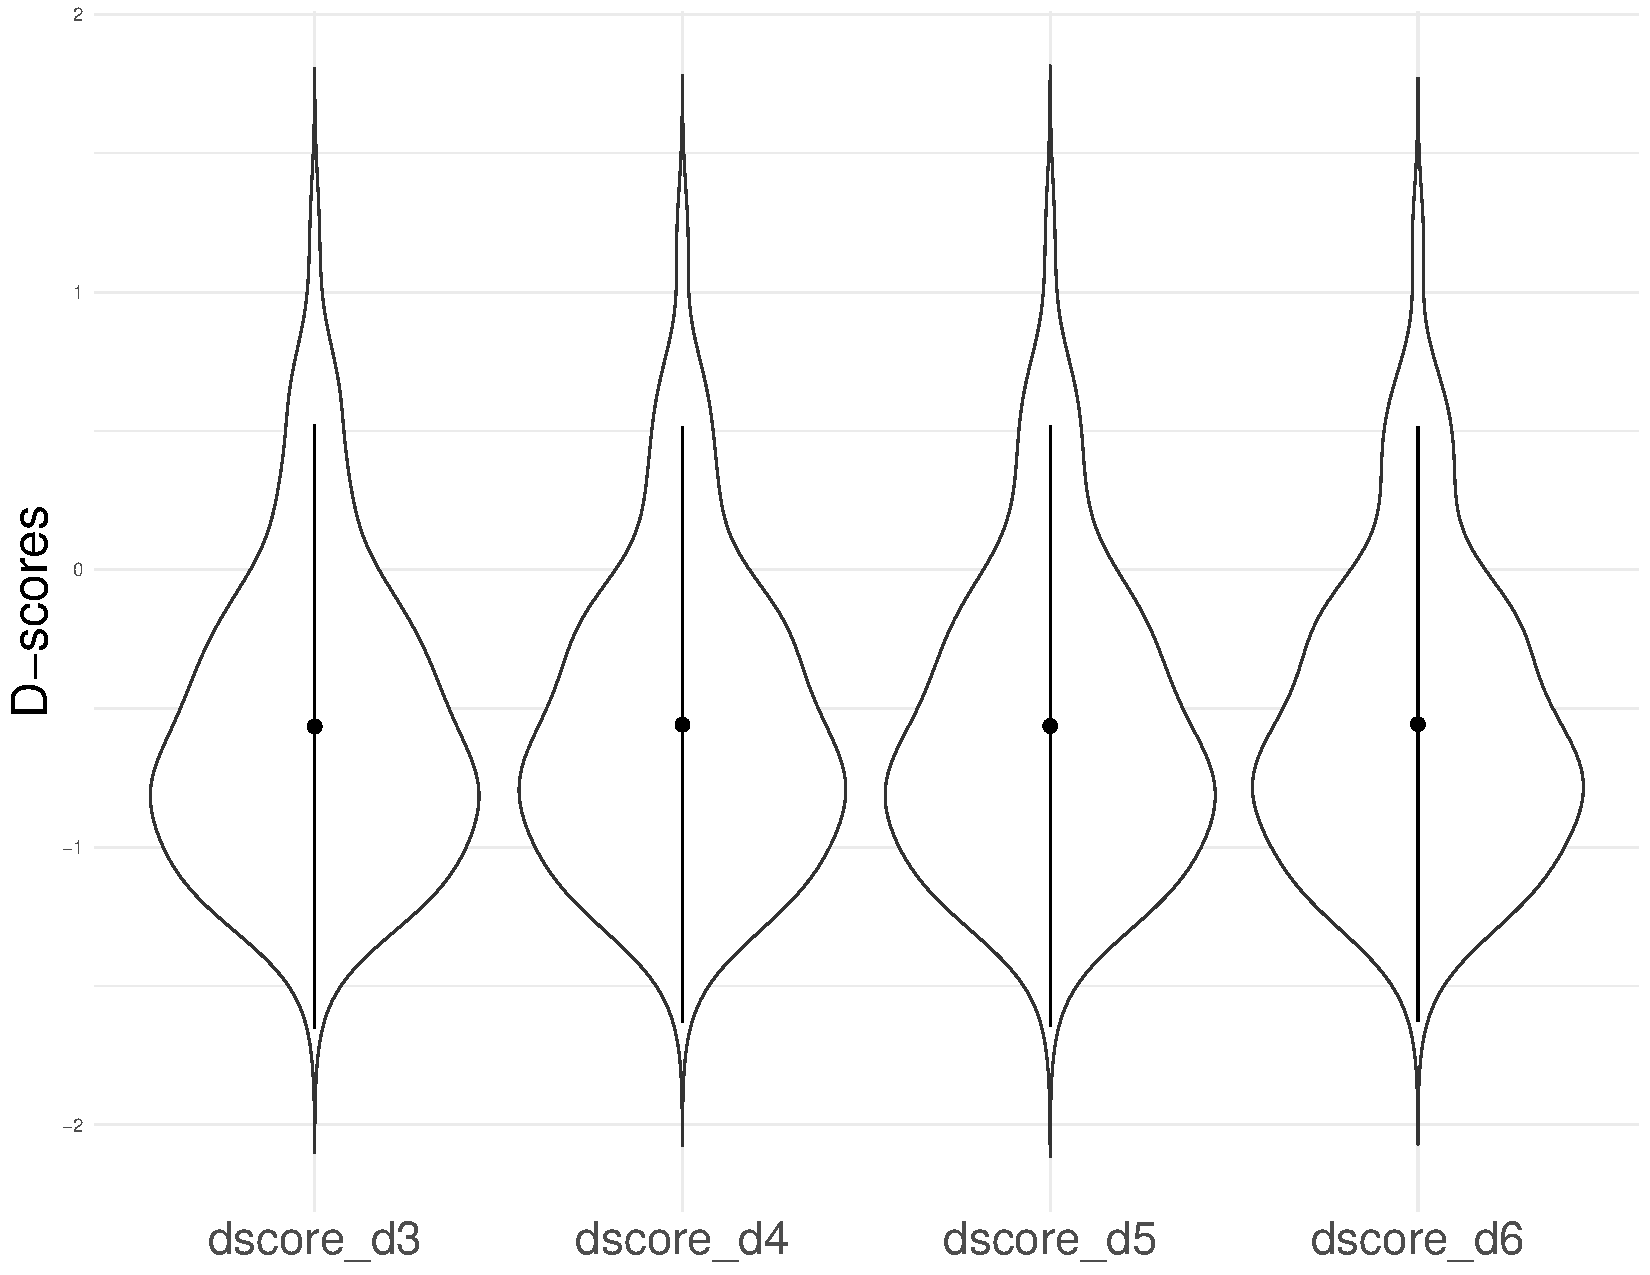
\includegraphics[width=0.5\linewidth]{multid.pdf}}  \\
	\end{tabular}


 
\vfill\null
\columnbreak

\begin{center}
	\huge \textbf{\textcolor{title}{SC-IAT example}}
\end{center}

The \texttt{raw\_data} toy data set contains data from two distinct data SC-IATs. Data from both SC-IATs can be simulatenously clenaed and prepared for the computation by using \textcolor{purple}{\texttt{clean\_sciat()}} function: 

\begin{lstlisting}
data("raw_data") # load toy data 
sciat_data <- clean_sciat(raw_data, # raw data set
                      sbj_id = "Participant", #Column with respondents' IDs
                      block_id = "blockcode", #Column with blocks labels
                      latency_id = "latency", #Column with latency responses
                      accuracy_id = "correct", #Column with accuracy responses
                      block_sciat_1 = c("test.sc_dark.Darkbad", #1st SC-IAT block labels
                      "test.sc_dark.Darkgood"),
                      block_sciat_2 = c("test.sc_milk.Milkbad", #2nd SC-IAT block labels
                      "test.sc_milk.Milkgood"),
                      trial_id  = "trialcode", #Column with trial labels
                      trial_eliminate = c("reminder", 
                      "reminder1")) #Trials to eliminate
\end{lstlisting}	

The object resulting from \textbf{\textcolor{purple}{\texttt{clean\_sciat()}}} is a list containing two data sets of class \textcolor{purple}{\texttt{sciat\_clean}}, one for each SC-IAT. These data sets can be individually passed to \textbf{\textcolor{purple}{\texttt{Dsciat()}}} for the computation of the SC-IAT \emph{D-score}: 
\begin{lstlisting}
 d_sciat1 <- Dsciat(sciat_data[[1]], # 1st SC-IAT data
                   mappingA = "test.sc_dark.Darkbad", # Mapping A Label
                   mappingB = "test.sc_dark.Darkgood", # Mapping B Label
                  non_response = "alert") # Label for responses over rtw
 d_sciat2 <- Dsciat(sciat_data[[2]], # 2nd SC-IAT data
                   mappingA = "test.sc_milk.Milkbad", # Mapping A Label
                   mappingB = "test.sc_milk.Milkgood", # Mapping B Label
                   non_response = "alert") # Label for responses over rtw
\end{lstlisting}	

The objects obtained from \textbf{\textcolor{purple}{\texttt{Dsciat()}}} function have class \textcolor{purple}{\texttt{dsciat}} and they can be passed to functions \textbf{\textcolor{purple}{\texttt{descript\_d()}}}, \textbf{\textcolor{purple}{\texttt{d\_plot()}}}, and \textbf{\textcolor{purple}{\texttt{d\_distr()}}}, as the objects obtained from \textbf{\textcolor{purple}{\texttt{computeD()}}} function. 

Results obtained from multiple SC-IATs can be plotted together by using \textcolor{purple}{\texttt{multi\_dsciat()}}: 

\begin{tabular}{c c}
	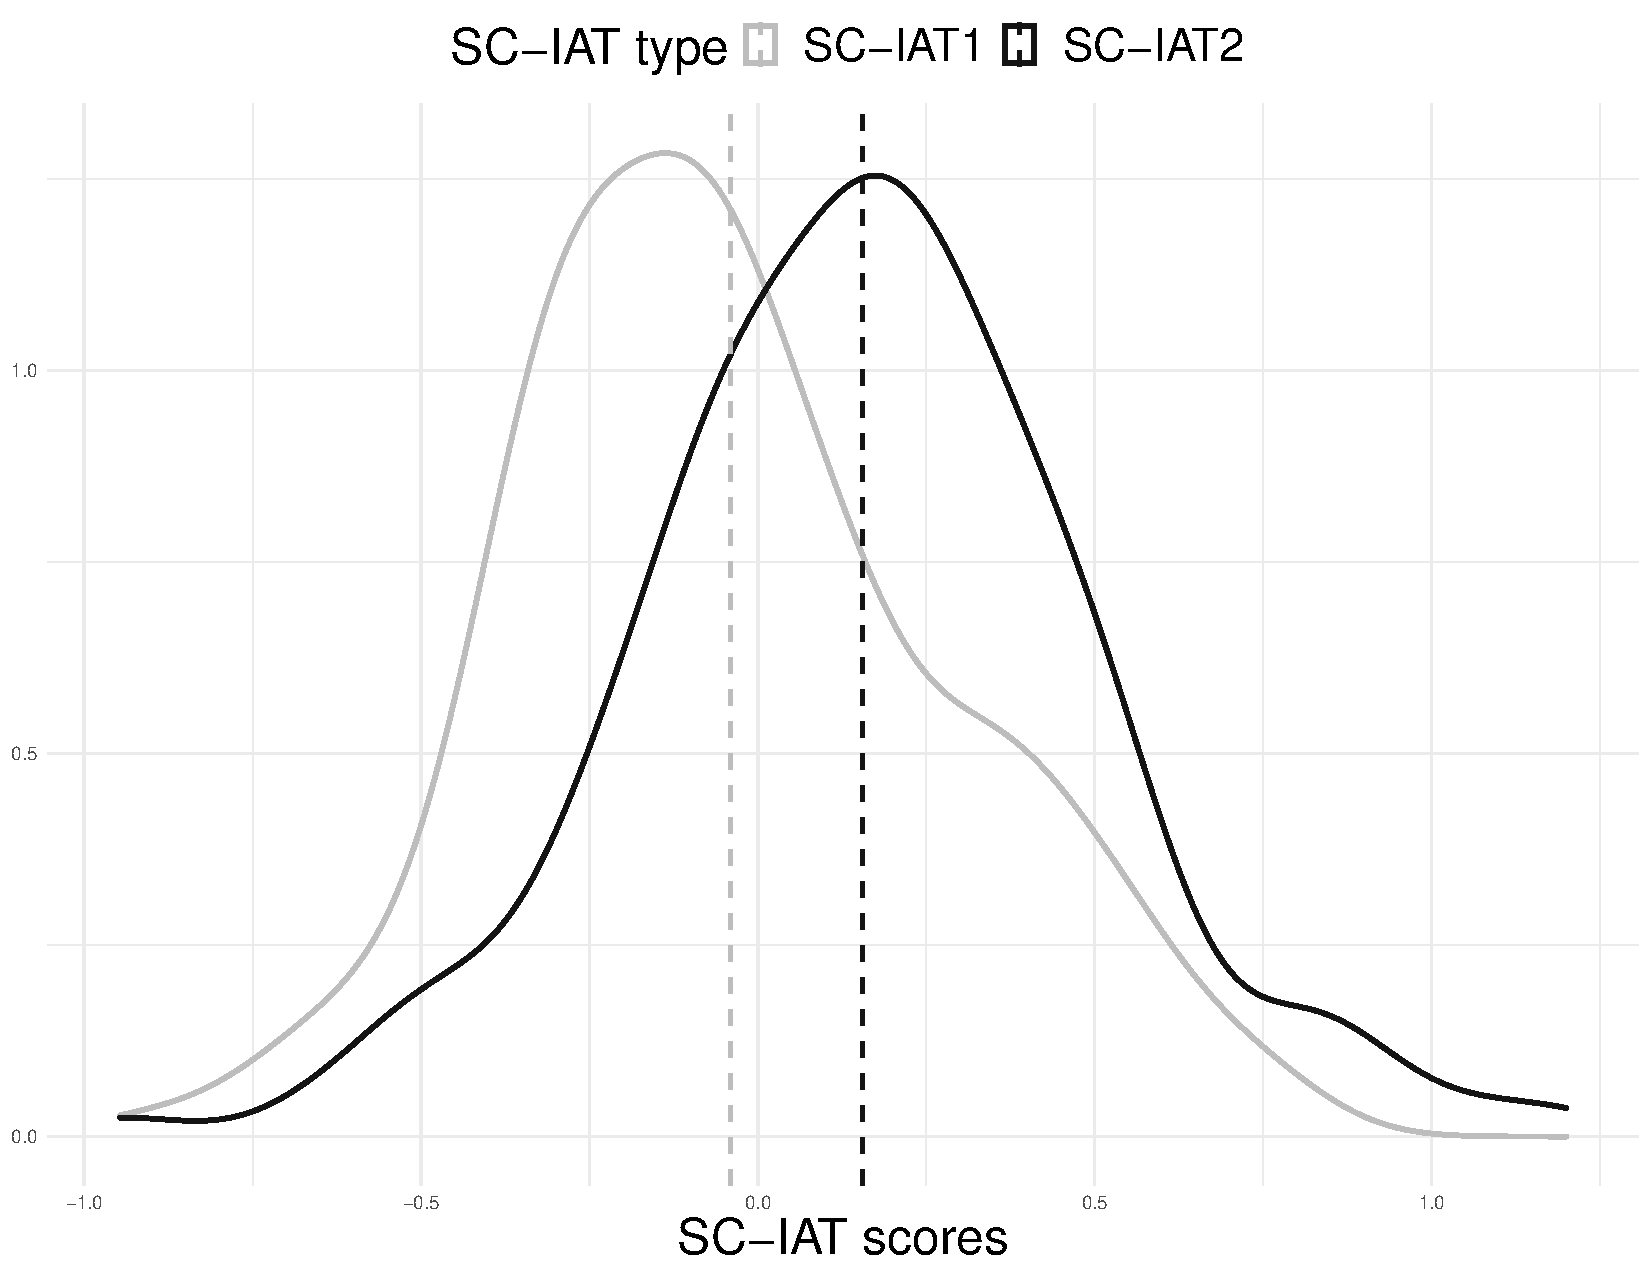
\includegraphics[width=0.5\linewidth]{sciatDefault.pdf}
	&
	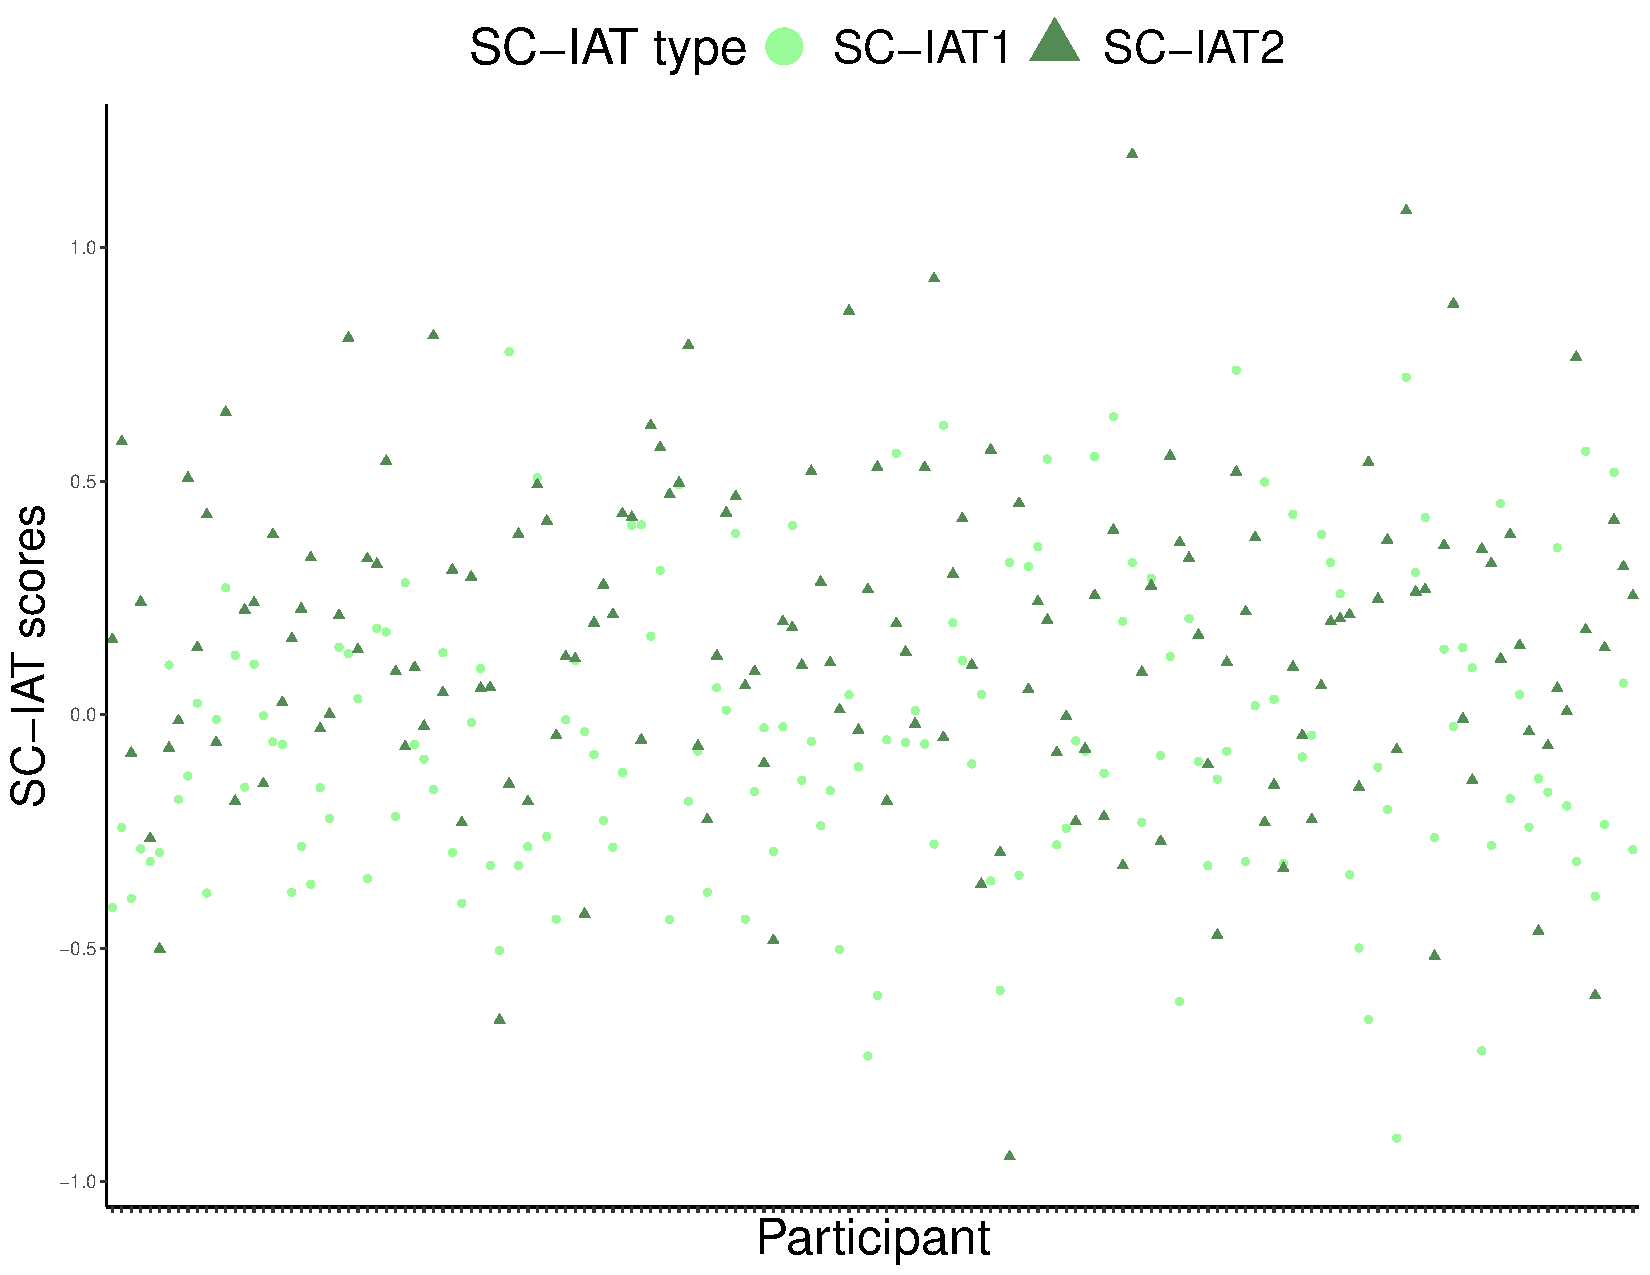
\includegraphics[width=0.5\linewidth]{multiSciatPoints.pdf} \\
	\textbf{\textcolor{purple}{\texttt{multi\_dsciat()}}}  Default settings & \textbf{\textcolor{purple}{\texttt{multi\_dsciat()}}} Customized plot\\
\end{tabular}

\vspace{5mm}

\textcolor{title}{Last but not least:} All graphical functions are based on \texttt{ggplot2} \cite{ggplot2} and can be further modified by the users! 

\vspace{5mm}
---------------------------------------
\footnotesize
%\nocite{*} % Print all references regardless of whether they were cited in the poster or not
\bibliographystyle{plain} % Plain referencing style
\bibliography{poster} % Use the example bibliography file sample.bib

%----------------------------------------------------------------------------------------

\end{multicols*}
\end{document}